
\chapter{Implementation}
\section{Overview}
\section{Hyper parameters}
\subsection{Clear Every Step}

\subsection{Gradient Method}

\subsection{Gradient Threshold Considered}

\subsection{Multiply Weight }

\subsection{Proxy Steps}

\subsection{Subset Of Wrongly Classified}

\section{Data Loading and Pre Processing}
\subsection{Directory structure}

\subsection{Label function}

\subsection{Clearing proxy images}

\subsection{Encode, Stratify, Kfold}

\subsection{train and test, val separate}

\subsection{Augmentations}
Imagenet Normalize
Tensor
Num workers

\section{Training Details}

\section{Grid Search}

\section{Optimizations}
\subsection{Mixed Precision}
\subsection{Gradient Scaling}
\subsection{No grad}
\subsection{Batched Proxy step}
\subsection{Trial Resumption}


\subsection{Models}
TIMM

\section{Gradient Based Methods}
\section{Proxy Attention}

% \begin{algorithm}
%     \caption{Calculate $y = x^n$}

%     % \caption{Proxy Attention Single Batch}
%     \begin{algorithmic}[1]
%         \Require $config, input_wrong, cam$
%         % \Function{proxy_one_batch}{$config, input_wrong, cam$}
%         \State $grads \gets$ \Call{$cam$}{$input_wrong.to(config["device"]), None$}
%         \State $grads \gets$ \Call{$torch.Tensor$}{$grads$}$.\Call{to}{config["device"]}$.
%         $unsqueeze(1).\Call{expand}{-1, 3, -1, -1}$
%         \State $normalized_inps \gets$ \Call{$inv_normalize$}{$input_wrong$}
%         \If{$config["pixel_replacement_method"] \neq "blended"$}
%         \State $output \gets$ \Call{$torch.where$}{$grads > config["proxy_threshold"],$\
%         \hskip\algorithmicindent\hskip\algorithmicindent\hskip\algorithmicindent
%         \Call{$dict_decide_change$}{$config["pixel_replacement_method"], grads$},\
%         \hskip\algorithmicindent\hskip\algorithmicindent\hskip\algorithmicindent
%         $normalized_inps$}
%         \Else
%         \State $output \gets$ \Call{$torch.where$}{$grads > config["proxy_threshold"],$\
%         \hskip\algorithmicindent\hskip\algorithmicindent\hskip\algorithmicindent
%         $(1 - config["proxy_image_weight"] * grads) * normalized_inps$,\
%         \hskip\algorithmicindent\hskip\algorithmicindent\hskip\algorithmicindent
%         $normalized_inps$}
%         \EndIf
%         % \EndFunction
%         \end{algorithmic}
% \end{algorithm}

\subsection{Callback Mechanism}
\section{Tensorboard}
\section{Transfer learning}
\section{Optimizer}
\section{LR scheduler}
\section{Loss function}
\section{Batch sizer finder}
To maximize training performance, a batch size finder is used to find the optimal batch size for each of the models. 

\begin{algorithm}
    % \caption{Calculate $y = x^n$}

    \caption{Batch Size Finder Algorithm}
    \begin{algorithmic} 
        \REQUIRE $dataset\_size, max\_batch\_size, failed$
        \STATE $batch\_size = 2$
        \WHILE{TRUE}
            \IF{$max\_batch\_size$ is not $None$ \And$ $batch\_size \geq max\_batch\_size$}
                \STATE $batch\_size \leftarrow max\_batch\_size$
            \ENDIF
            \IF{$batch\_size \geq dataset\_size$}
                \STATE $batch\_size \leftarrow batch\_size // 2$
            \ENDIF

            \IF{$failed$ is $False$}
                \LOOP
                    \STATE $inputs \leftarrow random((batch\_size,input\_shape))$
                    \STATE $targets \leftarrow random((batch\_size,output\_shape))$
                    \STATE $outputs \leftarrow model(inputs)$
                    \STATE $loss \leftarrow MSE(outputs, targets)$
                    \STATE $loss.backward()$
                    \STATE $optimizer.step()$
                    \STATE $optimizer.zero\_grad()$
                    \STATE $failed \leftarrow True$
                    \STATE $batch\_size \leftarrow batch\_size * 2$
                \ENDLOOP
            \ELSIF{$failed$ is $True$}
                \STATE $failed \leftarrow False$
                \STATE $batch\_size \leftarrow batch\_size // 2$
            \ENDIF

        \ENDWHILE

    \end{algorithmic}
    % \REQUIRE $n \geq 0 \vee x \neq 0$
    % \ENSURE $y = x^n$
    % \STATE $y \leftarrow 1$
    % \IF{$n < 0$}
    % \STATE $X \leftarrow 1 / x$
    % \STATE $N \leftarrow -n$
    % \ELSE
    % \STATE $X \leftarrow x$
    % \STATE $N \leftarrow n$
    % \ENDIF
    % \WHILE{$N \neq 0$}
    % \IF{$N$ is even}
    % \STATE $X \leftarrow X \times X$
    % \STATE $N \leftarrow N / 2$
    % \ELSE[$N$ is odd]
    % \STATE $y \leftarrow y \times X$
    % \STATE $N \leftarrow N - 1$
    % \ENDIF
    % \ENDWHILE
    % \end{algorithmic}
\end{algorithm}

% \begin{algorithm}
% \caption{Batch Size Finder Algorithm}
% \begin{algorithmic}
% \State $batch\_size = 2$
% \State $max\_batch\_size = None$
% \State $dataset\_size = len(dataset)$
% \While{True}
% \If{$max\_batch\_size$ is not None and $batch\_size \geq max\_batch\_size$}
% \State $batch\_size = max\_batch\_size$
% \EndIf

% \If{$batch\_size$ \geq $dataset\_size$}
% \State $batch\_size = batch\_size//2$
% \EndIf

% \EndWhile
% \end{algorithmic}
% \end{algorithm}

% \begin{figure}[h]
% 	\centering
% 	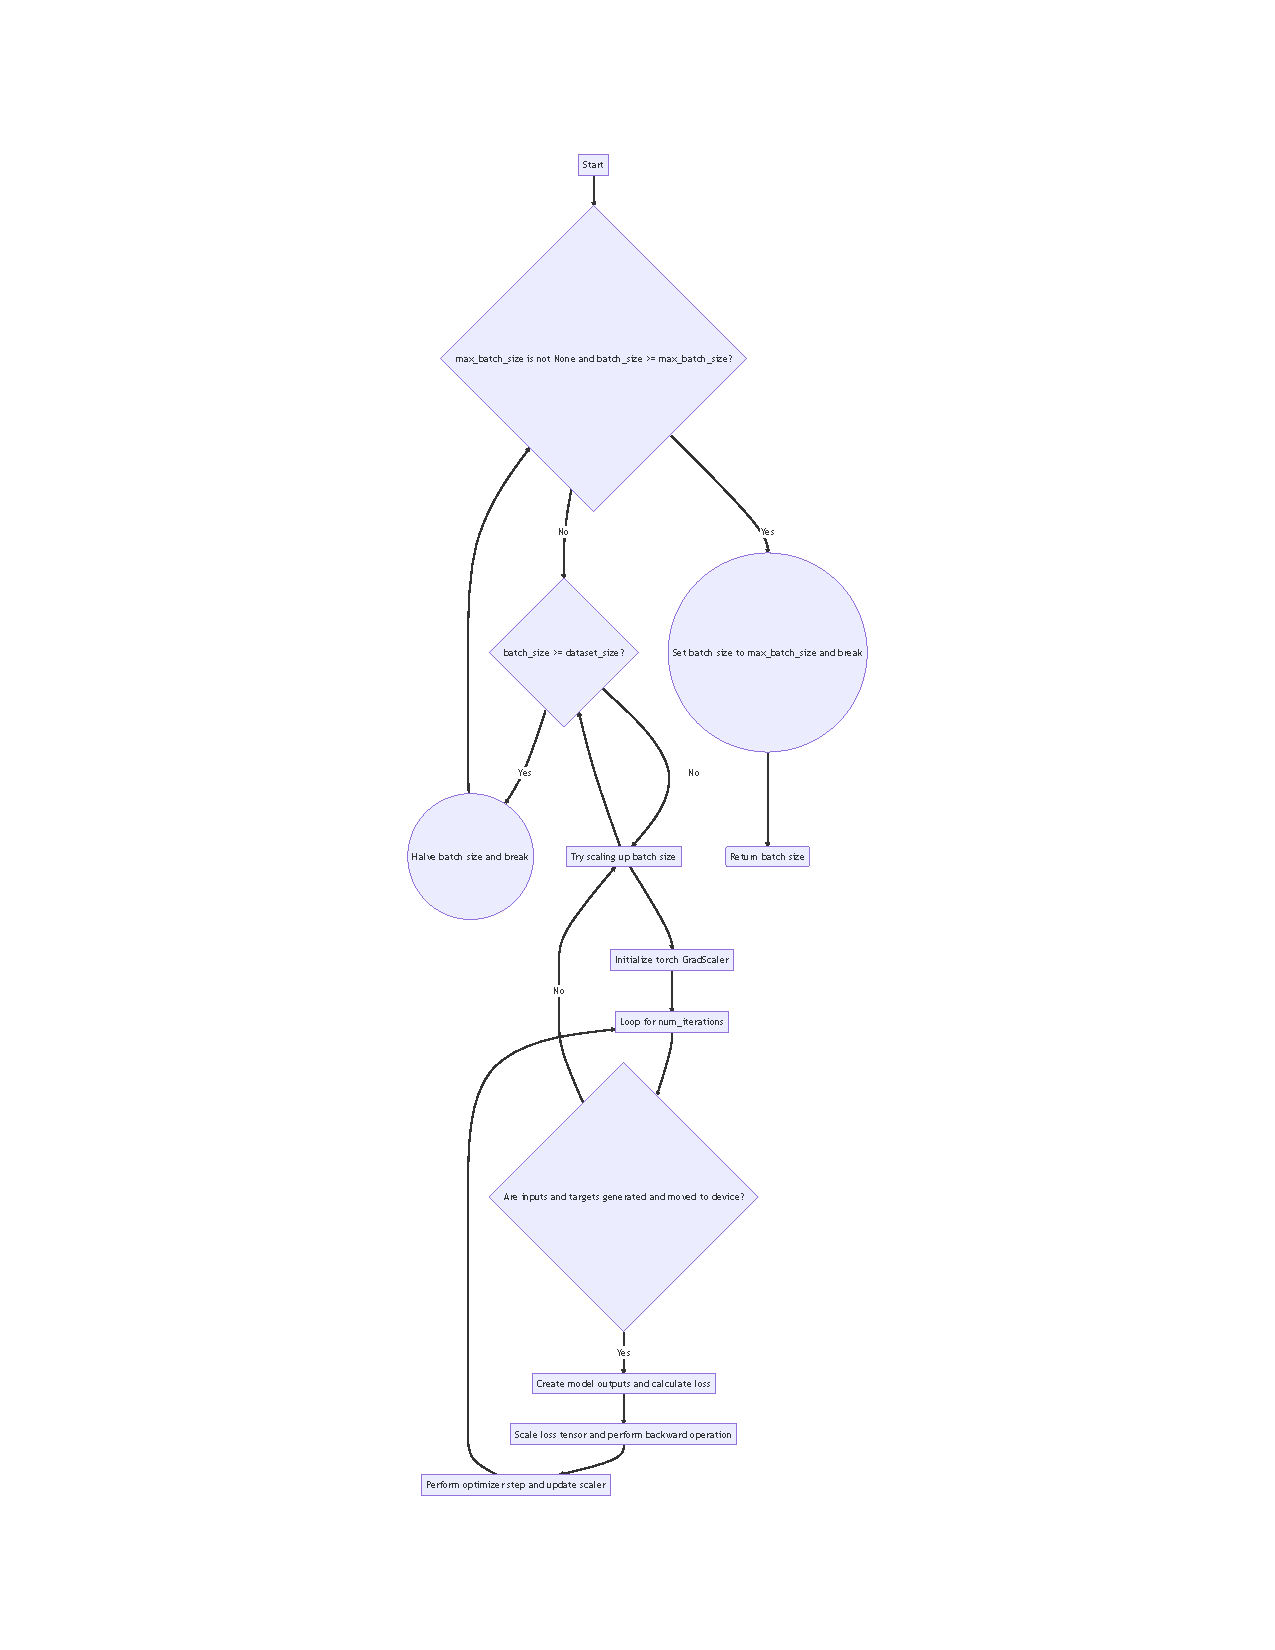
\includegraphics[width=0.8]{images/bsfinder.pdf}
% 	\caption{Batch Size Finder Algorithm}
% 	\label{fig:bsfind}
% \end{figure}
\section{Result Aggregation}

\section{Inference}